\documentclass[11pt]{article}

\usepackage[margin=1in]{geometry}
\usepackage{amsmath,amssymb,booktabs,longtable,array}
\usepackage{graphicx}
\usepackage{hyperref}
\usepackage{natbib}
\usepackage{enumitem}
\usepackage{microtype}

\title{RAPM DECOMP: An Additive Decomposition of Regularized Adjusted Plus-Minus}
\author{Russell Thomas}
\date{Draft of May 2026}

\begin{document}
\maketitle

\begin{abstract}
Regularized adjusted plus-minus is powerful because it estimates player impact
while controlling for the other nine players on the floor.  It is also hard to
trust as a public explanation because the usual output is a single coefficient.
This paper introduces RAPM DECOMP, an additive framework that opens the RAPM
coefficient into possession-value channels while preserving the adjusted-lineup
discipline that makes RAPM useful.  The central idea is simple: construct
component targets on the same possession surface, verify the arithmetic before
interpretation, solve each target with the same lineup-adjusted ridge operator,
and test whether the resulting factors add back to the actual offensive and
defensive RAPM coefficients.

The public RAPM DECOMP surface decomposes the actual offensive and defensive
RAPM coefficients into EFG value, free-throw value, turnover value, and
second-chance value.  The EFG value branch is the shot-value branch: it is
reported as a rolled-up factor and can be opened into an internal baseline plus
rim, midrange, and three-point frequency and conversion atoms.  Free-throw value
is divided into trip frequency and trip severity.  Turnover value is expressed
in points, not merely as a turnover-rate coefficient, so it can be added to
scoring terms.  On the current 2024--2026 NBA public export,
797 player rows and 7.73 million
possession-weighted player observations have maximum rounded residual 0.001
points per 100 possessions between actual RAPM and the factor sum, with
possession-weighted mean absolute residual 0.000255.  The long 1997--2026
export contains 2,859 player rows and 71.03 million possession-weighted
observations with the same maximum rounded residual.  The
result is not a claim that basketball causality is solved.  It is a claim that
RAPM can be made less silent: the adjusted signal can be assigned to transparent
possession channels with almost zero public accounting error.
\end{abstract}

\section{Introduction}

Basketball statistics are often split into two unsatisfying families.  Box-score
and tracking-based statistics can explain what happened in basketball
terms, but they can miss effects that appear only through teammates, opponents,
spacing, screening, rotations, and lineup context.
Adjusted plus-minus models control for teammates and opponents, but they usually
return a single number.  That single number is useful, but it is quiet.  A
player can have a large RAPM coefficient because his lineups generate better
shots, draw more valuable free throws, avoid turnovers, crush second chances,
suppress rim value, or combine several smaller effects.  The coefficient itself
does not say which channels carried the value.

RAPM DECOMP is an attempt to keep the strength of RAPM while opening the
coefficient into basketball terms.  The method does not regress a player-level
RAPM rating on box-score summaries.  It stays at the possession level, where
RAPM is estimated.  Each component is a mechanically defined target attached to
the same lineup rows.  The model then asks: if the dependent variable is shot
value instead of total point differential, which players are associated with
that shot value after controlling for teammates and opponents?  The same
question is asked for free throws, turnovers, and second chances.

The key constraint is additivity.  Public decomposition columns should not be
mere labels placed beside a total coefficient.  They should be in common units,
with an explicit test against the parent coefficient.  The current public RAPM
DECOMP export does this in points per 100 possessions.  On offense, the
first-chance structure is:
\[
\text{oFC}
= \text{oEFG}
+ \text{oFT}
+ \text{oTOV}.
\]
Here \texttt{oFC} is offensive first-chance RAPM: effective-field-goal value,
free-throw value, and turnover value before the first offensive rebound.  Total
offense then adds second-chance value:
\[
\text{off}
= \text{oFC}
+ \text{oSC}.
\]
Here \texttt{oEFG} is offensive effective-field-goal value, \texttt{oFT} is
offensive free-throw value, \texttt{oTOV} is offensive turnover value, and
\texttt{oSC} is offensive second-chance value.  The scoring sum
\texttt{oEFG + oFT} is \texttt{oTS}: an adjusted first-chance points-per-shot
RAPM term, so \texttt{oFC = oTS + oTOV}.  The same structure holds for defense:
\texttt{dEFG + dFT + dTOV = dFC}, with \texttt{dTS = dEFG + dFT}.  Defensive
terms mean effective-field-goal prevention, free-throw prevention, turnover
creation, and second-chance prevention after sign-flipping defensive factors so
that positive is good for the player's team.  The validation residual is not a
fifth basketball term.  It is the measured difference between actual RAPM and
the factor sum, and the point of the paper is that this difference is
almost zero in the public exports.

This paper makes three contributions.  First, it defines an additive
RAPM-decomposition operator: component targets are solved with the same
lineup-adjusted ridge machinery as total RAPM.  Second, it gives a basketball
schema for the largest scoring channels: first-chance shot value, free-throw
value, first-chance turnover value, and second-chance value, with shot value
reported publicly as \texttt{oEFG}/\texttt{dEFG} and opened into a baseline
closure term plus location-frequency and location-conversion atoms.  Third, it
reports
the residual between actual RAPM and the factor sum in current public exports
and shows player profiles that are recognizable as basketball rather than as
arbitrary post-processing.

\section{Background}

Adjusted plus-minus treats a stint or possession as an observation and the
players on the floor as signed predictors.  Ridge regularization stabilizes the
estimate in the presence of repeated lineups, collinearity, and low-minute
players.  The resulting RAPM coefficient is a partial association between a
player and team scoring margin, conditional on the other players in the row.
This conditional structure is the core reason RAPM matters.

RAPM also has well-known limits.  Players are not randomly assigned to lineups.
Roles, coaches, teammates, opponents, score effects, and era effects all matter.
Regularization reduces variance, but it does not create a randomized
experiment.  RAPM should therefore be read as adjusted evidence, not as a pure
causal treatment effect.

The usual public workaround is to blend adjusted plus-minus with box-score,
tracking, or scouting priors.  Those hybrids can be excellent rating systems,
but they answer a different question from decomposition.  A prior-centered
metric asks how to stabilize a player rating.  RAPM DECOMP asks where the
adjusted rating lands in the possession economy.  Priors can later be attached
to each channel, but the channel itself should have a mechanical target.

The method also differs from a box-score explanation layer.  A player-level
summary such as rim attempts, assists, turnover percentage, or offensive
rebound rate can help explain a component, but it is not the component.  The
component is estimated from lineup-adjusted possession outcomes.  For example,
offensive rim-frequency value is not simply the player's own rim-attempt rate.
It is the adjusted value of lineups shifting first-chance shot value toward or
away from the rim while that player is on offense.

\section{Related Work and Motivation}

The public lineage begins with adjusted plus-minus: estimate player effects from
scoring margin while controlling for all players on the floor.  Rosenbaum's
early public work introduced the broad idea to basketball audiences, and Sill's
regularized formulation made the approach more practical by using shrinkage and
out-of-sample testing.  Later possession-value models, including work by
Cervone, D'Amour, Bornn, and Goldsberry, showed that basketball possessions can
be valued as evolving states rather than only as final outcomes.

RAPM DECOMP sits between those traditions.  Like RAPM, it uses lineup-adjusted
estimation rather than assigning credit directly from the event log.  Like
possession-value work, it insists that the scoreboard can be opened into smaller
states and events.  The distinct move is to keep the RAPM design matrix and
change the target.  The model does not ask which player recorded a box-score
event.  It asks which players are associated with possession-value channels
after the same teammate and opponent controls used in RAPM.

The immediate predecessor is a six-factor adjusted-plus-minus layer.  That layer
solves separate adjusted factors for scoring efficiency, turnovers, and
rebounding on offense and defense.  It is useful because it demonstrates that
large portions of RAPM can be spanned by broad basketball families.  The current
2021--2026 time-decayed six-factor export reconstructs total RAPM at
$R^2=0.985745$ with a possession-weighted mean absolute residual of 0.201
points per 100 possessions.  That is already a strong result: shooting,
turnovers, and rebounding are not just box-score labels; they are adjusted
lineup channels.

But the six-factor layer also shows why a stricter additive layer is needed.
True-shooting value, turnover rate, and rebounding rate do not naturally live on
the same denominator or in the same units.  A public table can use a
second-stage regression to translate them, but the reader is still looking at a
model of a model.  RAPM DECOMP makes the scoring branch more direct.  It uses
point-valued component targets on a shared possession frame, then publishes
component values that are already in the same units as total RAPM.

The motivation is therefore not to replace broad-factor RAPM.  The broad layer
is a useful map.  RAPM DECOMP is a more exact accounting surface underneath the
largest and most semantically crowded part of that map: how scoring value is
created, lost, extended, and suppressed.

\section{RAPM as an Operator}

Let $j$ index possession rows.  Let $y_j$ be a target, such as total point
differential, shot value, free-throw value, turnover value, or second-chance
value.  Let $w_j$ be an observation weight.  Let $X$ be the sparse player design
matrix.  In a simplified single-block notation, $X_{jp}=+1$ when player $p$ is
on the offensive side of row $j$, $X_{jp}=-1$ when player $p$ is on the
defensive side, and $X_{jp}=0$ otherwise.
Production solves use separate offensive and defensive columns and can apply
different penalties by side, but the notation is enough to state the idea.
The ridge estimate is
\[
\hat{\beta}_y =
\arg\min_{\beta}
\sum_j w_j (y_j - X_j\beta)^2 + \lambda \|\beta\|_2^2 .
\]
Define $R(y)=\hat{\beta}_y$, the regularized lineup-adjustment operator applied
to target $y$.

If a row target decomposes as
\[
y = a + b + c,
\]
one might hope that $R(y)=R(a)+R(b)+R(c)$.  This is not the identity on which
RAPM DECOMP relies.  Separate ridge solves, recentering, nuisance terms, and
rounded CSV exports can perturb raw coefficient sums even when row algebra is
exact.  RAPM DECOMP therefore measures the residual directly:
\[
\text{Residual} = R(y) - \sum_k R(c_k),
\]
where $R(y)$ is the actual parent RAPM coefficient and $R(c_k)$ are the factor
coefficients.  In other words: build component targets that have a clear
arithmetic relationship, solve them consistently, and show that the actual
parent coefficient is reconstructed by the factor sum.

This ordering matters.  A component coefficient is meaningful only if the target
it came from is meaningful.  If the row construction is wrong, a tidy player
table is not evidence.  If the row construction is sound but factor
coefficients do not add back to the actual parent coefficient, the difference
is the decomposition error.  The public claim here is that this error is almost
zero in the finished exports.

\section{The Decomposition Tree}

The public RAPM DECOMP table uses a nested decomposition.  At the top level:
\[
\text{RAPM}
\rightarrow
\text{Offense} + \text{Defense}.
\]
Within each side:
\[
\text{Actual Side RAPM}
\rightarrow
\text{EFG Value}
+ \text{Free-Throw Value}
+ \text{Turnover Value}
+ \text{Second-Chance Value}.
\]
The parent is the actual published side coefficient: \texttt{off} for offense
and \texttt{def} for defense.  The factor sum is checked against that parent;
it is not a substitute metric.

Shot value has two levels.  The public \texttt{oEFG}/\texttt{dEFG} factor is
the rolled-up first-chance non-free-throw shot-value channel.  Inside that
channel, the value above the average first-chance shot is split into six atoms:
\[
\text{EFG Value Atoms}
= \text{Rim Frequency} + \text{Rim Conversion}
+ \text{Midrange Frequency} + \text{Midrange Conversion}
+ \text{Three-Point Frequency} + \text{Three-Point Conversion}.
\]
The rolled-up public factor is:
\[
\text{EFG Value}
= \text{EFG Baseline}
+ \text{EFG Value Atoms}.
\]
Free-throw value is split as:
\[
\text{Free-Throw Value}
= \text{Trip Frequency Value} + \text{Trip Severity Value}.
\]
Turnover value is split as:
\[
\text{Turnover Value}
= \text{Bad-Pass Turnover Value}
+ \text{Scoring Turnover Value}.
\]

\subsection{First Chance and Second Chance}

The temporal division is central.  First-chance value is the offense's value
before the first offensive miss.  Second-chance value is the value after that
first offensive miss.  This avoids hiding post-miss scoring inside a first-shot
metric and avoids confusing offensive rebounding with the points that follow an
extended possession.

A true first-chance turnover is a possession-ending turnover before a
first-chance shot or free-throw completion.  If a possession already produced a
make, field-goal attempt, or completed free-throw sequence, a later terminal
turnover does not retroactively erase that first-chance scoring.  This guard is
small in code and large in meaning: the same possession should not be counted
both as realized first-chance scoring and as lost first-chance scoring value.

\subsection{EFG Value}

The public \texttt{oEFG} and \texttt{dEFG} factors are not ordinary effective
field-goal percentage.  They are point-valued first-chance non-free-throw shot
targets on the shared possession surface.  The public rolled-up factor includes
both a baseline shot-value term and the six location atoms.  The location atoms
measure value above or below an average first-chance shot, rather than crediting
a player merely for the existence of a shot.  The baseline term keeps the
unatomized part of first-chance EFG value inside the EFG branch, so it is not
misassigned to free throws, turnovers, second chance, or residual.

The frequency atoms price location mix.  Rim frequency is valuable when moving a
lineup's first-chance shot diet toward the rim has positive expected value
relative to the average first-chance shot.  Midrange frequency can be negative
when shifting toward midrange reduces value.  Three-point frequency can be
positive or negative depending on the loaded sample's shot-value environment.
The conversion atoms measure within-location make value after the average value
of that location has been priced.

\subsection{Free Throws}

Free-Throw Value is split into trip frequency and trip severity.  Frequency
credits the creation of first-chance free-throw trips at the average trip value
in the loaded sample.  Severity is the value above or below that average trip,
combining trip type and free-throw shooting.  The current split is intentionally
conservative: it separates creating trips from the value of those trips, but it
does not yet separate trip type from shooter conversion in the public table.

\subsection{Turnovers}

Turnover Value must be in points if it is to be added to shot and free-throw
components.  A rate-style turnover RAPM is useful, but it is not additive with
points.  RAPM DECOMP therefore prices true first-chance turnovers by the
first-chance scoring opportunity that was lost.  The parent turnover value is
then split into bad-pass turnover value and other scoring or ball-handling
turnover value.

This translation is one of the main reasons the factor sum can reconstruct
ORAPM cleanly.  A turnover is not treated as a negative shot.  It is treated as
the missing first-chance possession value that a non-turnover possession would
have produced on average in the relevant sample.

\section{Nuisance Terms and Public Units}

Production RAPM runs can include score-margin by period terms, season-phase
fixed effects, time decay, age terms, or other nuisance blocks.  These terms are
not basketball skill components.  They are included to keep player coefficients
from absorbing broad context shifts.  A public row must therefore be read with
its run specification.  The current primary NBA table used here is a
2024--2026 all-games run with score-margin adjustment, season-phase fixed
effects, and side-specific ridge penalties of 2000 on offense and 4000 on
defense.

The public file reports points per 100 possessions.  Defensive components are
sign-flipped so that positive values are good for the player's team.  This
gives the public convention:
\[
\text{Net RAPM} = \text{Offense} + \text{Defense},
\]
where positive offense and positive defense both mean positive player impact.

The player-facing component columns are centered by possession-weighted player
means on the published universe.  This does not change the underlying target.
It chooses a public zero.  The goal is readability: a value above zero means
above the published player baseline for that component and side.

\section{Implementation Workflow}

The production workflow has five steps.

\begin{enumerate}[leftmargin=*]
\item Build possession rows with offensive players, defensive players, game
metadata, and parent scoring targets.
\item Build component targets on those rows: shot value, free-throw value,
turnover value, second-chance value, and their child atoms.
\item Verify target arithmetic before fitting player coefficients.
\item Solve each target with the same RAPM machinery and the same stated run
controls.
\item Assemble a public weighted-factor table, sign-flip defense into a
good-positive convention, center component columns, and report the residual
between actual RAPM and the factor sum.
\end{enumerate}

The workflow deliberately separates three artifacts that are easy to conflate.
The processed possession files are the accounting surface.  The raw component
result files are separately regularized player estimates.  The public
weighted-factor file is the decomposition surface: it contains the actual
parent coefficients, the factor coefficients, and the residuals.  Each artifact
has a different job.  The processed files prove that the target is coherent.
The raw result files let an analyst audit each component solve.  The public file
is what a reader should use when asking whether the factors add to actual RAPM.

This is why the paper emphasizes public residuals.  A public decomposition
should not ask the reader to take additivity on faith.  It should show actual
RAPM, show the factors, and show actual RAPM minus the factor sum.  In the
finished five-year downstream export, that difference is zero at published CSV
precision for every player row.

\section{Validation}

RAPM DECOMP has two validation layers.  The first is target-level arithmetic.
The second is the public residual between actual RAPM and the factor sum.

\subsection{Target-Level Arithmetic}

The current processed 2024--2026 NBA surface verifies the internal EFG and
free-throw sub-identities to floating-point scale across 777,744 regular-season
and playoff possession rows.  Table \ref{tab:rowchecks} reports the maximum
absolute row gap and the number of rows with absolute gap greater than
$10^{-9}$.

\begin{table}[h]
\centering
\caption{Processed target sub-identity checks, 2024--2026 NBA rows}
\label{tab:rowchecks}
\begin{tabular}{lrr}
\toprule
Identity & Max absolute gap & Rows above $10^{-9}$\\
\midrule
Free throws = frequency + severity & $6.22\cdot10^{-15}$ & 0\\
Total EFG = baseline + EFG value & $5.68\cdot10^{-14}$ & 0\\
EFG value = rim + midrange + three & $8.88\cdot10^{-15}$ & 0\\
EFG value = six location atoms & $1.02\cdot10^{-14}$ & 0\\
Total EFG = baseline + six location atoms & $5.68\cdot10^{-14}$ & 0\\
\bottomrule
\end{tabular}
\end{table}

These checks are not model-fit statistics.  They are arithmetic checks on the
processed target surface.  Their purpose is to make sure the child targets mean
what the paper says they mean before any player coefficient is estimated.

\subsection{Public Export Residual}

The public RAPM DECOMP bundle then assembles solved component RAPMs into a
weighted-factor table.  Table \ref{tab:exports} summarizes three current
exports.  The six-factor row is included as a baseline: it reconstructs full
RAPM from independently solved shooting, turnover, and rebounding factors by a
second-stage weighted regression.  The RAPM DECOMP rows are public additive
bundles whose component columns are already in point-value units; the reported
residual is actual RAPM minus the factor sum.

\begin{table}[h]
\centering
\caption{Public reconstruction checks}
\label{tab:exports}
\begin{tabular}{lrrrr}
\toprule
Export & Players & Possession weight & $R^2$ & Max residual\\
\midrule
Six-factor 2021--2026 td700 & 1,086 & 15,160,930 & 0.985745 & 0.810\\
RAPM DECOMP 2024--2026 & 797 & 7,725,252 & 0.99999997 & 0.001\\
RAPM DECOMP 1997--2026 & 2,859 & 71,027,184 & 0.99999997 & 0.001\\
\bottomrule
\end{tabular}
\end{table}

The RAPM DECOMP residual is actual parent RAPM minus the factor sum.  On
offense:
\[
\text{oRESID}
= \text{off}
- (\text{oEFG}+\text{oFT}+\text{oTOV}+\text{oSC}).
\]
On defense the same definition applies with \texttt{def} and the defensive
factor columns.  The scientific claim is that the true ORAPM and DRAPM columns
are reconstructed by these factor sums with essentially no residual.

\subsection{What the Residual Means}

The residual is not a hidden fifth basketball component.  It is the error term
left after decomposing the actual parent RAPM coefficient into the published
point-valued factors.  A maximum residual of 0.001 points per 100 possessions is
too small to carry basketball interpretation.  It is rounding-scale
decomposition error.

This is different from the residual in the six-factor comparison.  The
six-factor residual is the unexplained portion of a second-stage reconstruction
from native-unit factor estimates.  It is meaningful because the factors are not
a direct point-valued decomposition of ORAPM and DRAPM.  The RAPM DECOMP
residual is smaller because the factors are constructed in the same units as
ORAPM and DRAPM, so the public test is direct: parent coefficient minus factor
sum.

The distinction matters for claims about "almost zero error."  The claim is not
that basketball is error-free or that every component is perfectly stable.  The
claim is that actual ORAPM and DRAPM decompose into the published factors with
only rounding-scale residual.  Statistical uncertainty remains in the component
estimates; decomposition residual is the part that has been driven close to
zero.

\section{Player Profiles}

Figures \ref{fig:jokic-shape}, \ref{fig:shai-shape}, and
\ref{fig:wembanyama-shape} are the most compact way to read RAPM DECOMP.  Each
player has eight bars: offense on the left, defense on the right, with a gap
between the sides.  Positive values go up; negative values go down.  The four
offensive bars add to ORAPM and the four defensive bars add to DRAPM up to the
reported residual.

\begin{figure}[h]
\centering
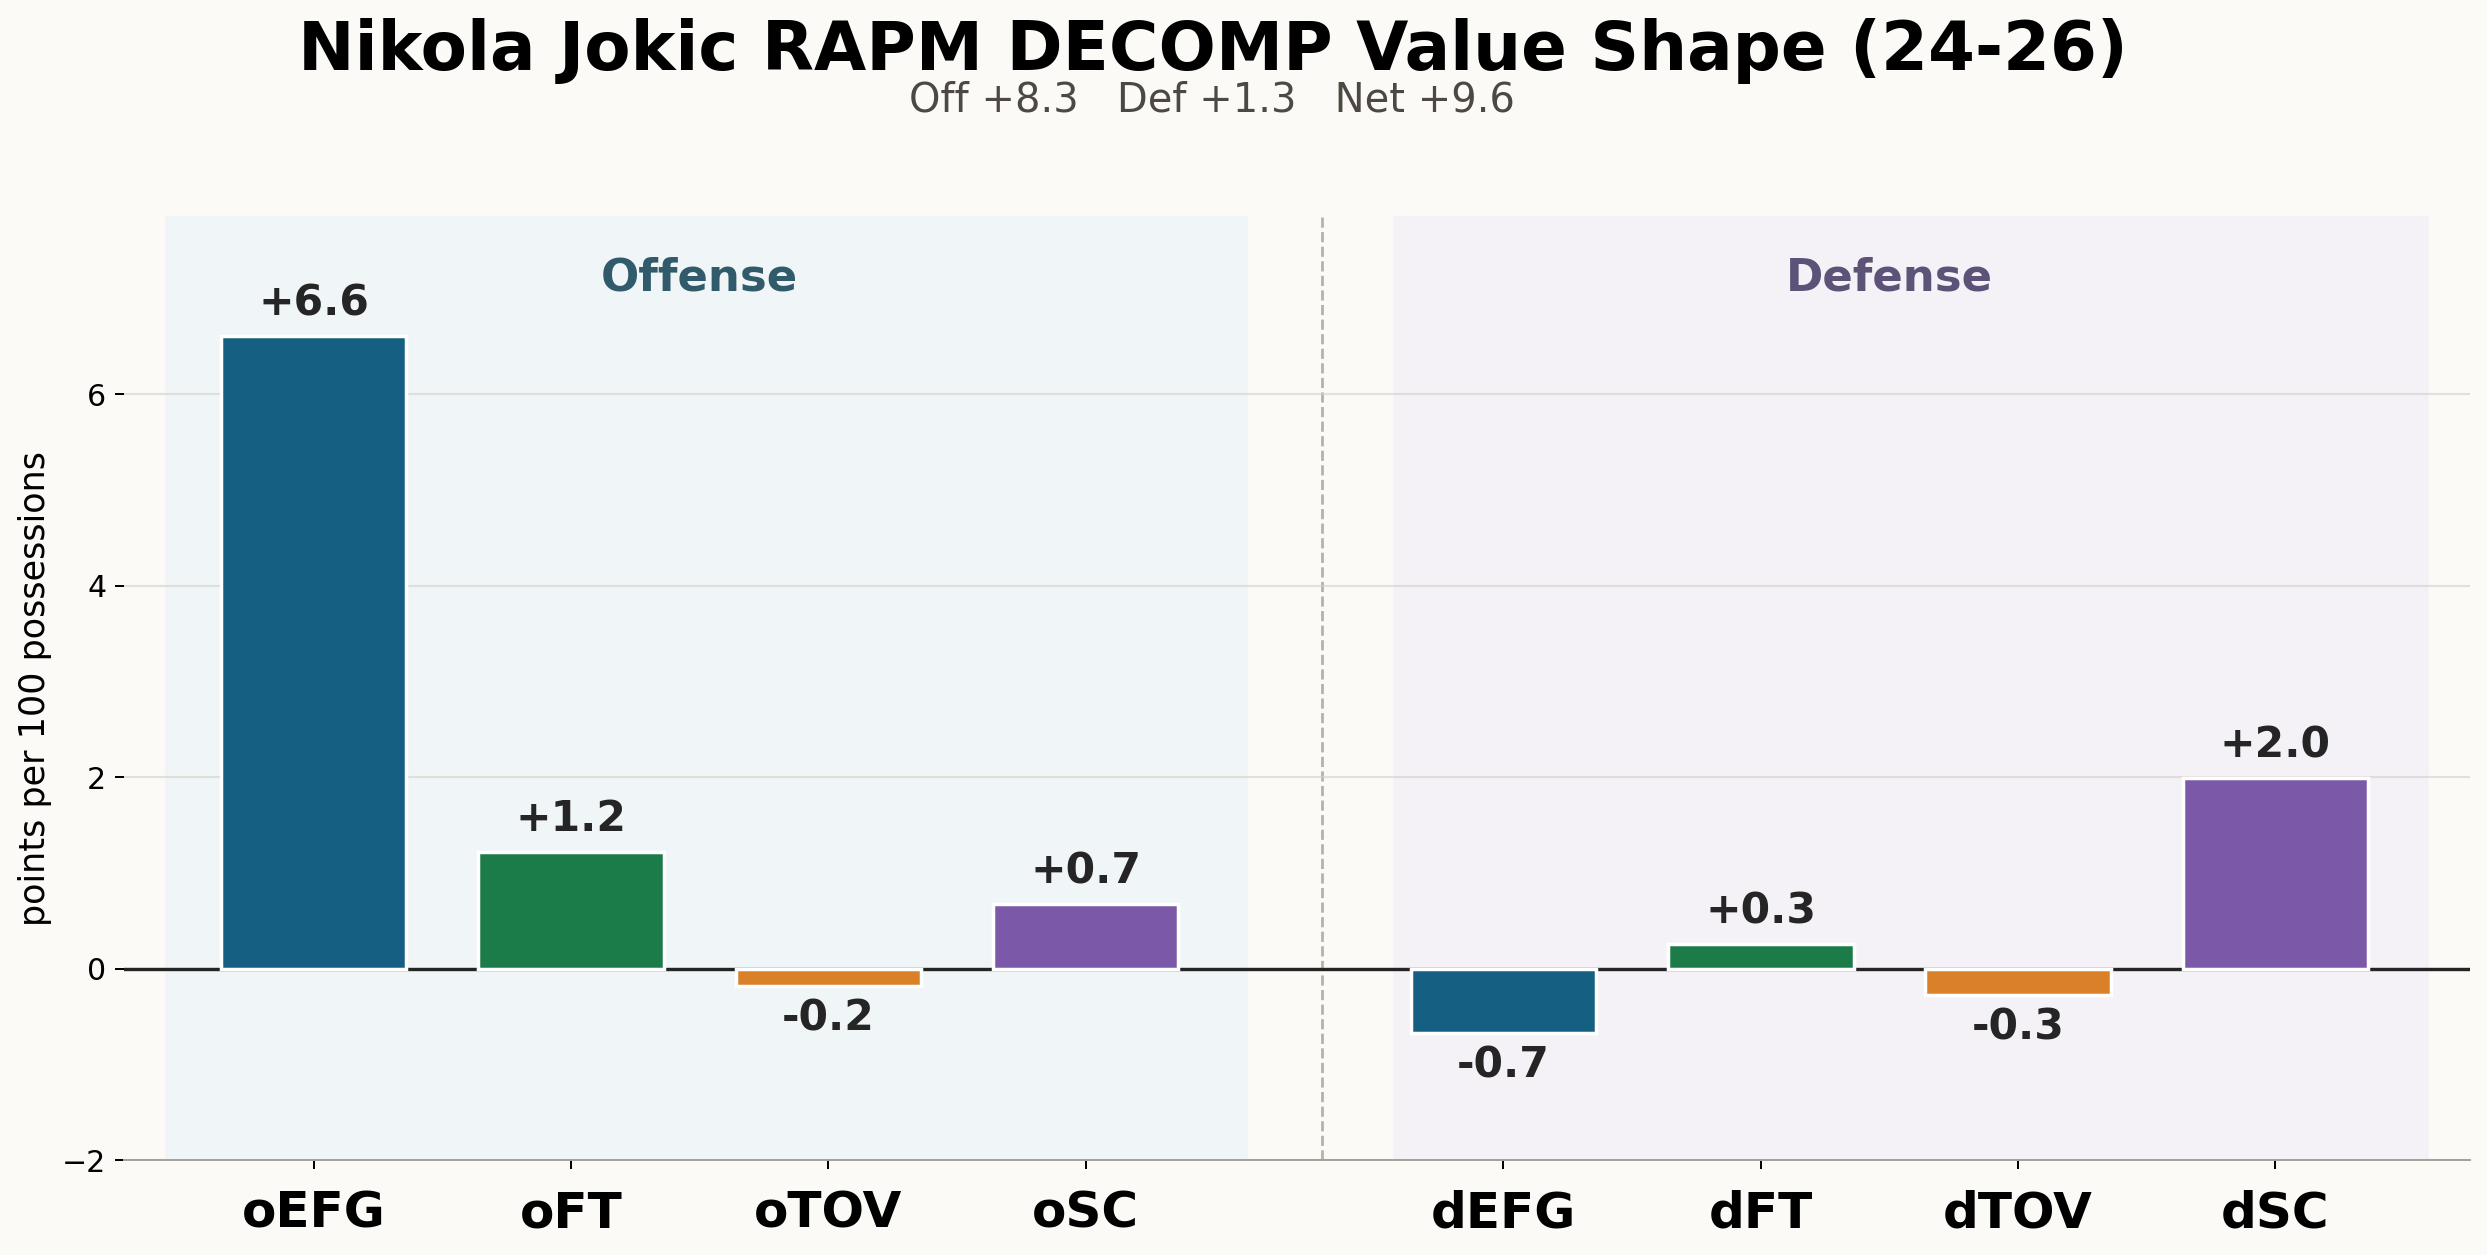
\includegraphics[width=0.92\linewidth]{figures/rapm_decomp_nikola_jokic_value_shape_24_26.png}
\caption{Nikola Jokic's 2024--2026 RAPM DECOMP value shape.  The left side
shows ORAPM factors; the right side shows DRAPM factors.}
\label{fig:jokic-shape}
\end{figure}

\begin{figure}[h]
\centering
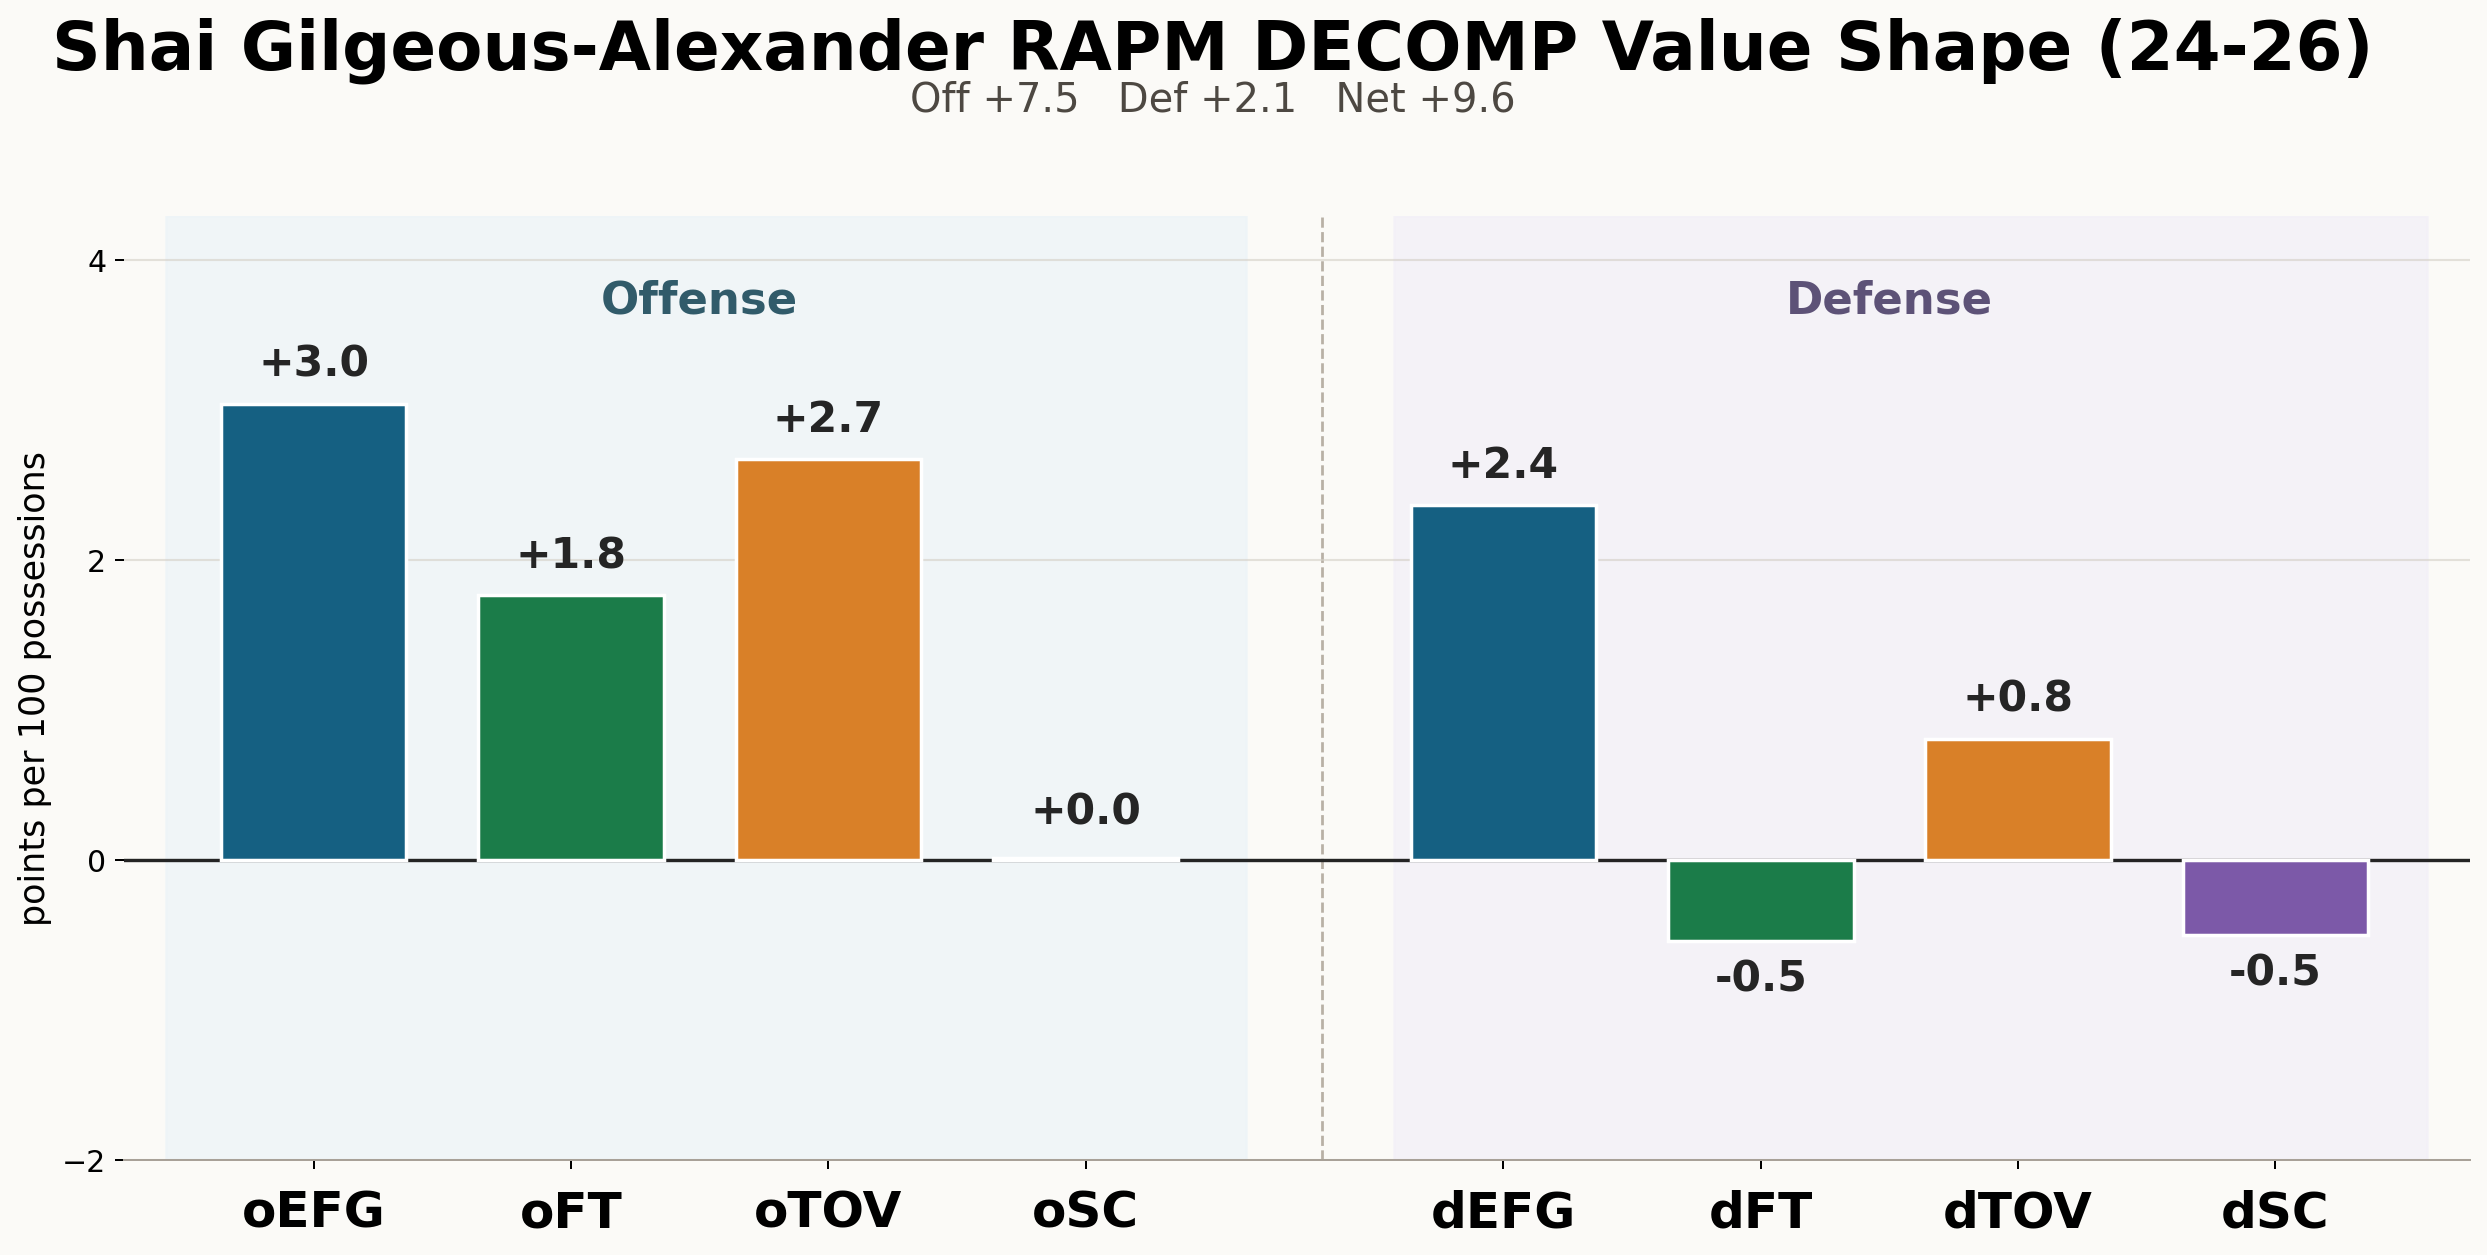
\includegraphics[width=0.92\linewidth]{figures/rapm_decomp_shai_gilgeous_alexander_value_shape_24_26.png}
\caption{Shai Gilgeous-Alexander's 2024--2026 RAPM DECOMP value shape.  The
offensive profile is much more balanced across EFG, FT, and turnover value than
Jokic's.}
\label{fig:shai-shape}
\end{figure}

\begin{figure}[h]
\centering
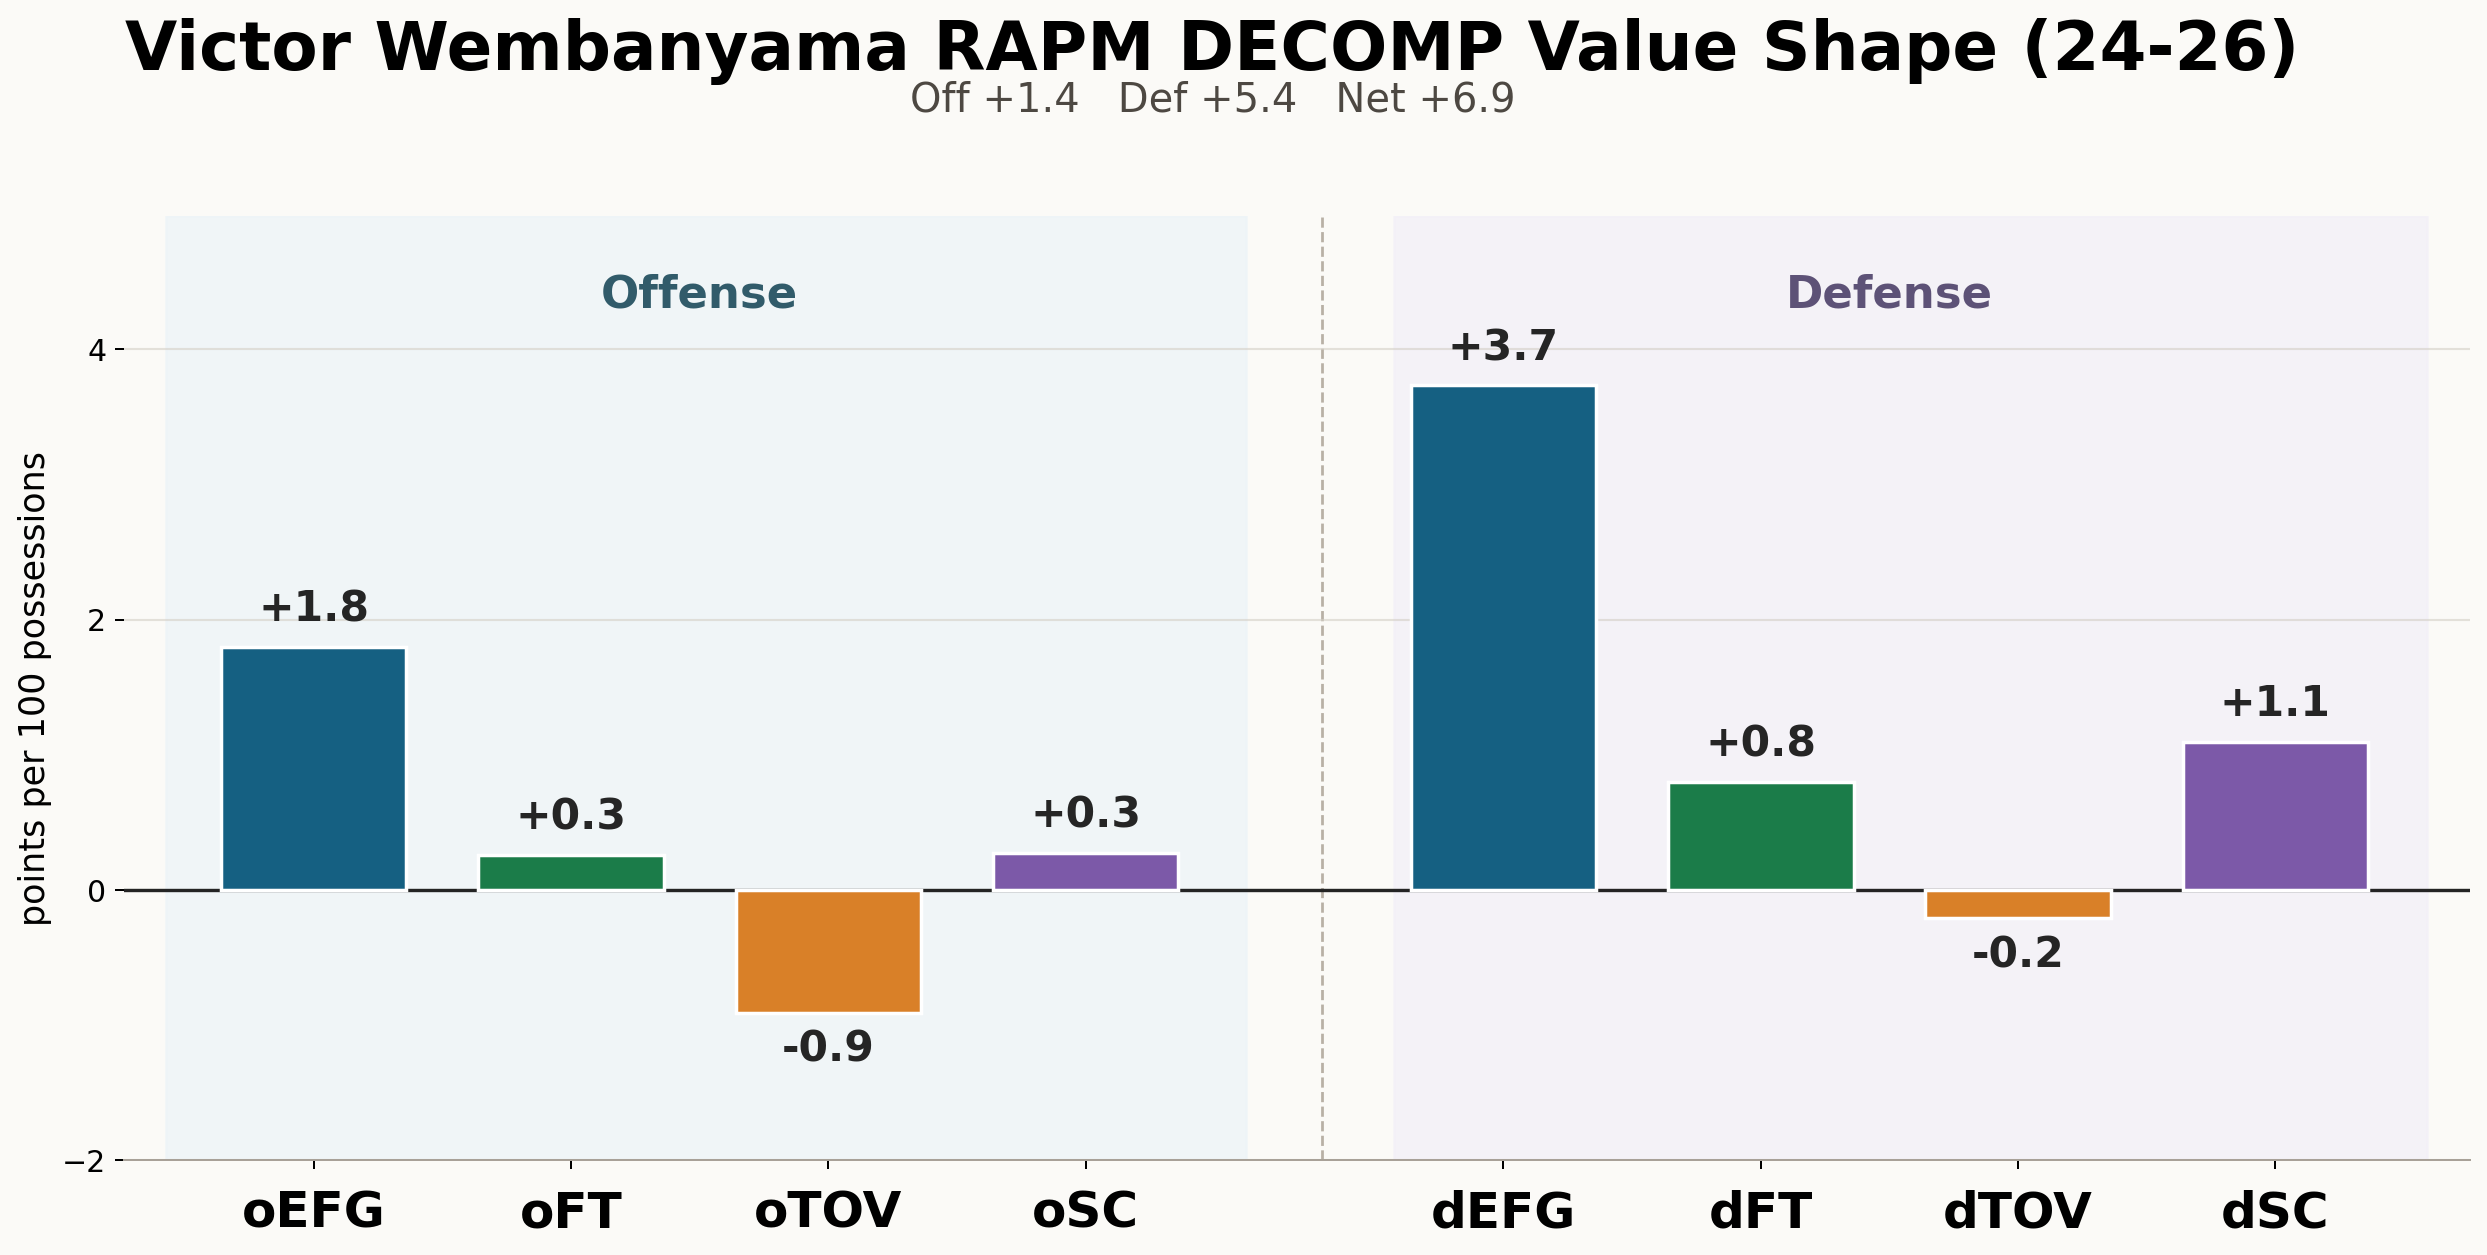
\includegraphics[width=0.92\linewidth]{figures/rapm_decomp_victor_wembanyama_value_shape_24_26.png}
\caption{Victor Wembanyama's 2024--2026 RAPM DECOMP value shape.  The chart
shows a defense-led profile with large \texttt{dEFG} and positive
second-chance defense.}
\label{fig:wembanyama-shape}
\end{figure}

Gilgeous-Alexander and Jokic have similar total values in this export, but their
profiles are not similar.  Gilgeous-Alexander's offensive value is spread across
\texttt{oEFG}, free throws, and first-chance turnover value.  Jokic's offensive
value is dominated by \texttt{oEFG}, with meaningful second-chance value and a
small negative first-chance turnover term.  RAPM DECOMP turns a one-number
comparison into a channel comparison without leaving the adjusted-plus-minus
framework.

Wembanyama illustrates the defensive side.  His total value is overwhelmingly
defensive, with a large \texttt{dEFG} bar, positive \texttt{dFT}, and positive
second-chance defense.  The same display format makes the contrast visible:
Jokic is an offense-led \texttt{oEFG} outlier, Gilgeous-Alexander is balanced
across offensive channels, and Wembanyama is a defense-led value shape.  These
statements are not film tags.  They are adjusted possession-channel estimates.

\subsection{A Worked Reading}

Consider Gilgeous-Alexander and Jokic.  A one-number RAPM table says both are
near the top of the league.  RAPM DECOMP says that the totals have different
shapes.  Gilgeous-Alexander's offensive profile combines \texttt{oEFG},
free-throw value, and a very large positive first-chance turnover-value term.
That last term should be read as possession preservation in point units, not
merely as a low turnover percentage.  Jokic's offense, by contrast, is dominated
by \texttt{oEFG}, with positive free-throw and second-chance value and a small
negative turnover-value term.  His lineups generate enormous first-chance
\texttt{oEFG} even after the opponent and teammate controls.

The defensive columns change the reading again.  Gilgeous-Alexander has a
positive \texttt{dEFG} coefficient in this export, while Jokic's public
\texttt{dEFG} component is negative and his defensive value is carried more by
second-chance defense and other terms.  That does not prove one player's
defensive mechanism by itself, but it tells the analyst where to look.  The
model turns "good" into a set of narrower questions.

The same pattern holds for Curry and Giannis.  Curry's shot value is mostly
conversion-led, especially from three.  Giannis's shot value is rim-led, with
large rim frequency and rim conversion value.  Those statements are not just
stylistic labels.  They are adjusted point-value channels that sum back to the
actual offensive RAPM coefficient.

\begin{table}[h]
\centering
\caption{Selected offensive EFG atoms, 2024--2026}
\label{tab:offshot}
\begin{tabular}{lrrrrrrr}
\toprule
Player & oEFG & RimFreq & RimConv & MidFreq & MidConv & 3Freq & 3Conv\\
\midrule
Nikola Jokic & 6.605 & 0.189 & 2.345 & 0.164 & 2.135 & 0.001 & 1.985\\
Stephen Curry & 5.601 & 0.283 & 1.281 & 0.685 & 0.750 & 0.012 & 2.630\\
Giannis Antetokounmpo & 5.225 & 0.719 & 2.746 & 0.785 & -0.483 & 0.017 & 1.242\\
Kevin Durant & 4.821 & -0.195 & 1.743 & -0.795 & 1.756 & 0.023 & 2.074\\
Tyrese Haliburton & 4.512 & -0.091 & 0.912 & 0.377 & 1.350 & 0.018 & 1.876\\
Jamal Murray & 3.706 & -0.216 & 0.212 & -0.366 & 1.163 & -0.003 & 2.616\\
Luka Doncic & 3.341 & -0.347 & 2.051 & 0.250 & 0.764 & 0.010 & 0.500\\
Shai Gilgeous-Alexander & 3.042 & -0.303 & 0.987 & -0.201 & 1.619 & 0.008 & 0.700\\
\bottomrule
\end{tabular}
\end{table}

The shot atoms keep one word, ``shooting,'' from doing too much work.  Curry's
largest atom is three-point conversion value.  Giannis combines large rim
frequency and rim conversion value while carrying negative midrange conversion
value.  Durant is negative by frequency mix and strongly positive by conversion.
Jokic has large positive conversion value in all three locations.  These are
lineup-adjusted possession-channel profiles, not simple shot charts.

\begin{table}[h]
\centering
\caption{Selected defensive EFG atoms, 2024--2026}
\label{tab:defshot}
\begin{tabular}{lrrrrrrr}
\toprule
Player & dEFG & RimFreq & RimConv & MidFreq & MidConv & 3Freq & 3Conv\\
\midrule
Rudy Gobert & 3.900 & 0.310 & 1.465 & 0.472 & 0.754 & -0.005 & 1.001\\
Victor Wembanyama & 3.735 & 0.352 & 1.497 & 0.120 & 0.891 & 0.009 & 1.002\\
Chet Holmgren & 2.906 & 0.205 & 2.059 & 0.206 & 0.362 & -0.000 & 0.174\\
Derrick White & 2.461 & 0.072 & 1.104 & 0.126 & 0.166 & 0.005 & 0.953\\
Shai Gilgeous-Alexander & 2.367 & 0.016 & 0.641 & -0.092 & 1.080 & -0.006 & 0.561\\
Jusuf Nurkic & 2.328 & 0.226 & 0.986 & 0.239 & 0.227 & 0.005 & 0.621\\
Marcus Smart & 1.646 & 0.166 & 0.530 & 0.094 & -0.247 & 0.010 & 1.086\\
\bottomrule
\end{tabular}
\end{table}

The defensive atom table separates location deterrence from conversion
suppression.  A rim protector may appear through rim conversion suppression,
through location mix, through second-chance value, or through a combination.
The decomposition does not identify every physical mechanism, but it prevents
all defensive value from being collapsed into one undifferentiated coefficient.

\section{Factor Geometry}

The factor correlations show that RAPM DECOMP is not merely a leaderboard with
extra columns.  The factors have structure.  In the 2024--2026 export, the main
offensive factors are related but not redundant: \texttt{oEFG} is positively
correlated with \texttt{oFT} and \texttt{oTOV}, while \texttt{oSC} moves in a
different direction.  On defense, \texttt{dFT} and \texttt{dTOV} are negatively
related in this player sample, and second-chance defense has its own shape.

\begin{figure}[h]
\centering
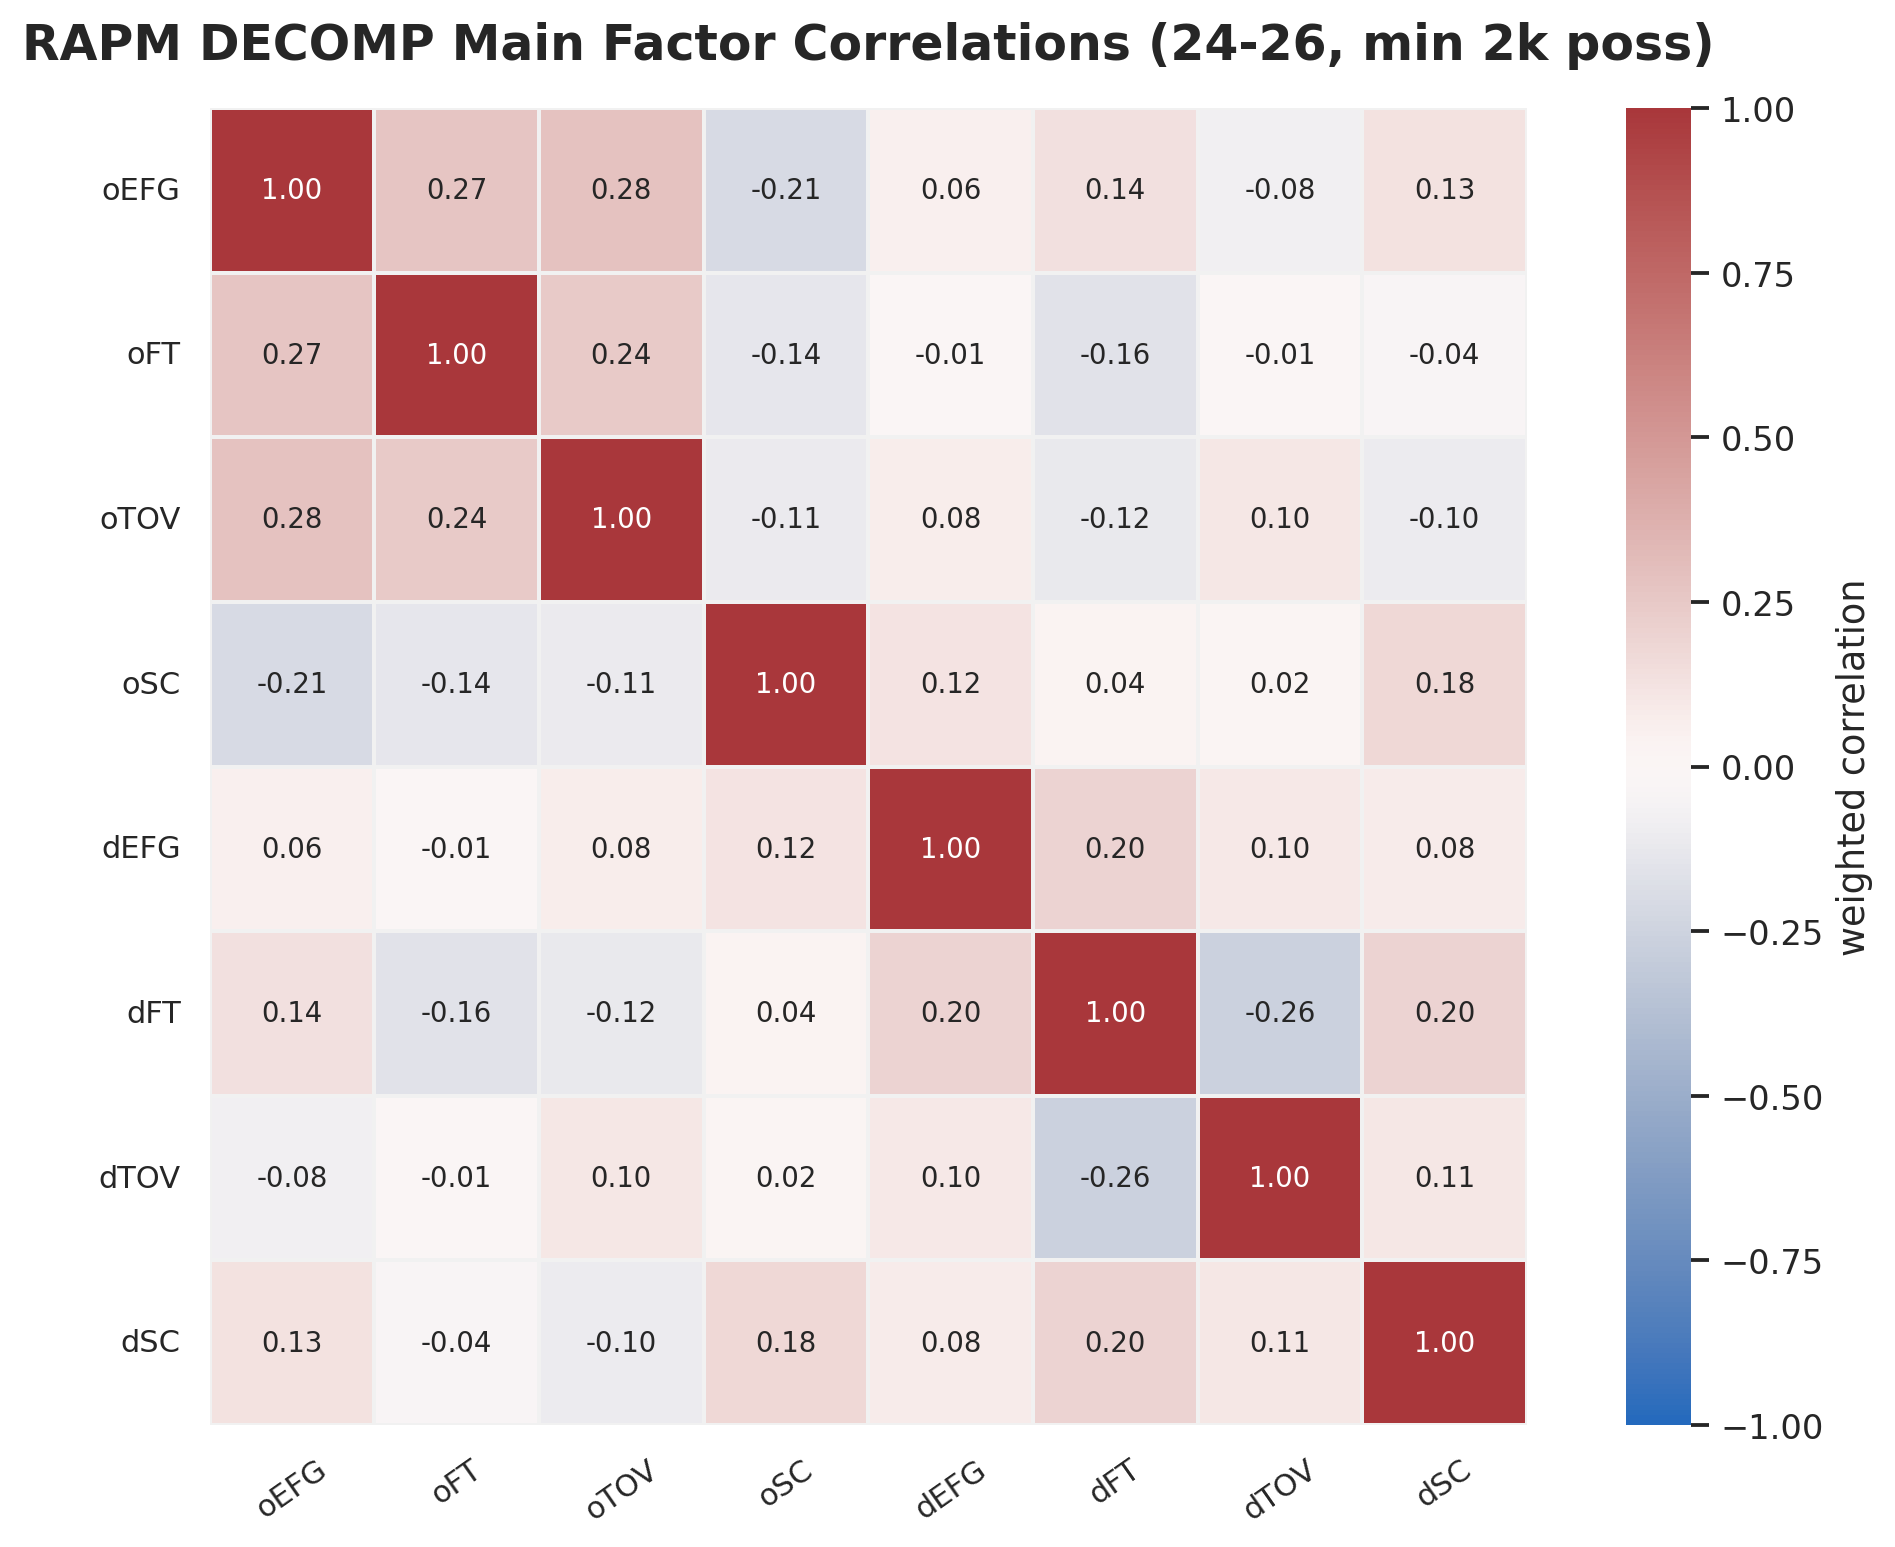
\includegraphics[width=0.92\linewidth]{figures/rapm_decomp_main_factor_corr_24_26.png}
\caption{Possession-weighted correlations among the eight main RAPM DECOMP
factors for 2024--2026 players with at least 2,000 possessions.}
\label{fig:main-corr}
\end{figure}

The atom-level views are more useful for scouting questions.  Offensive
midrange conversion travels with several creation and preservation signals, but
offensive second-chance value is not just another shooting column.  Defensively,
rim-frequency, rim-conversion, midrange-frequency, free-throw, and
second-chance columns show a coherent interior-defense cluster.

\begin{figure}[h]
\centering
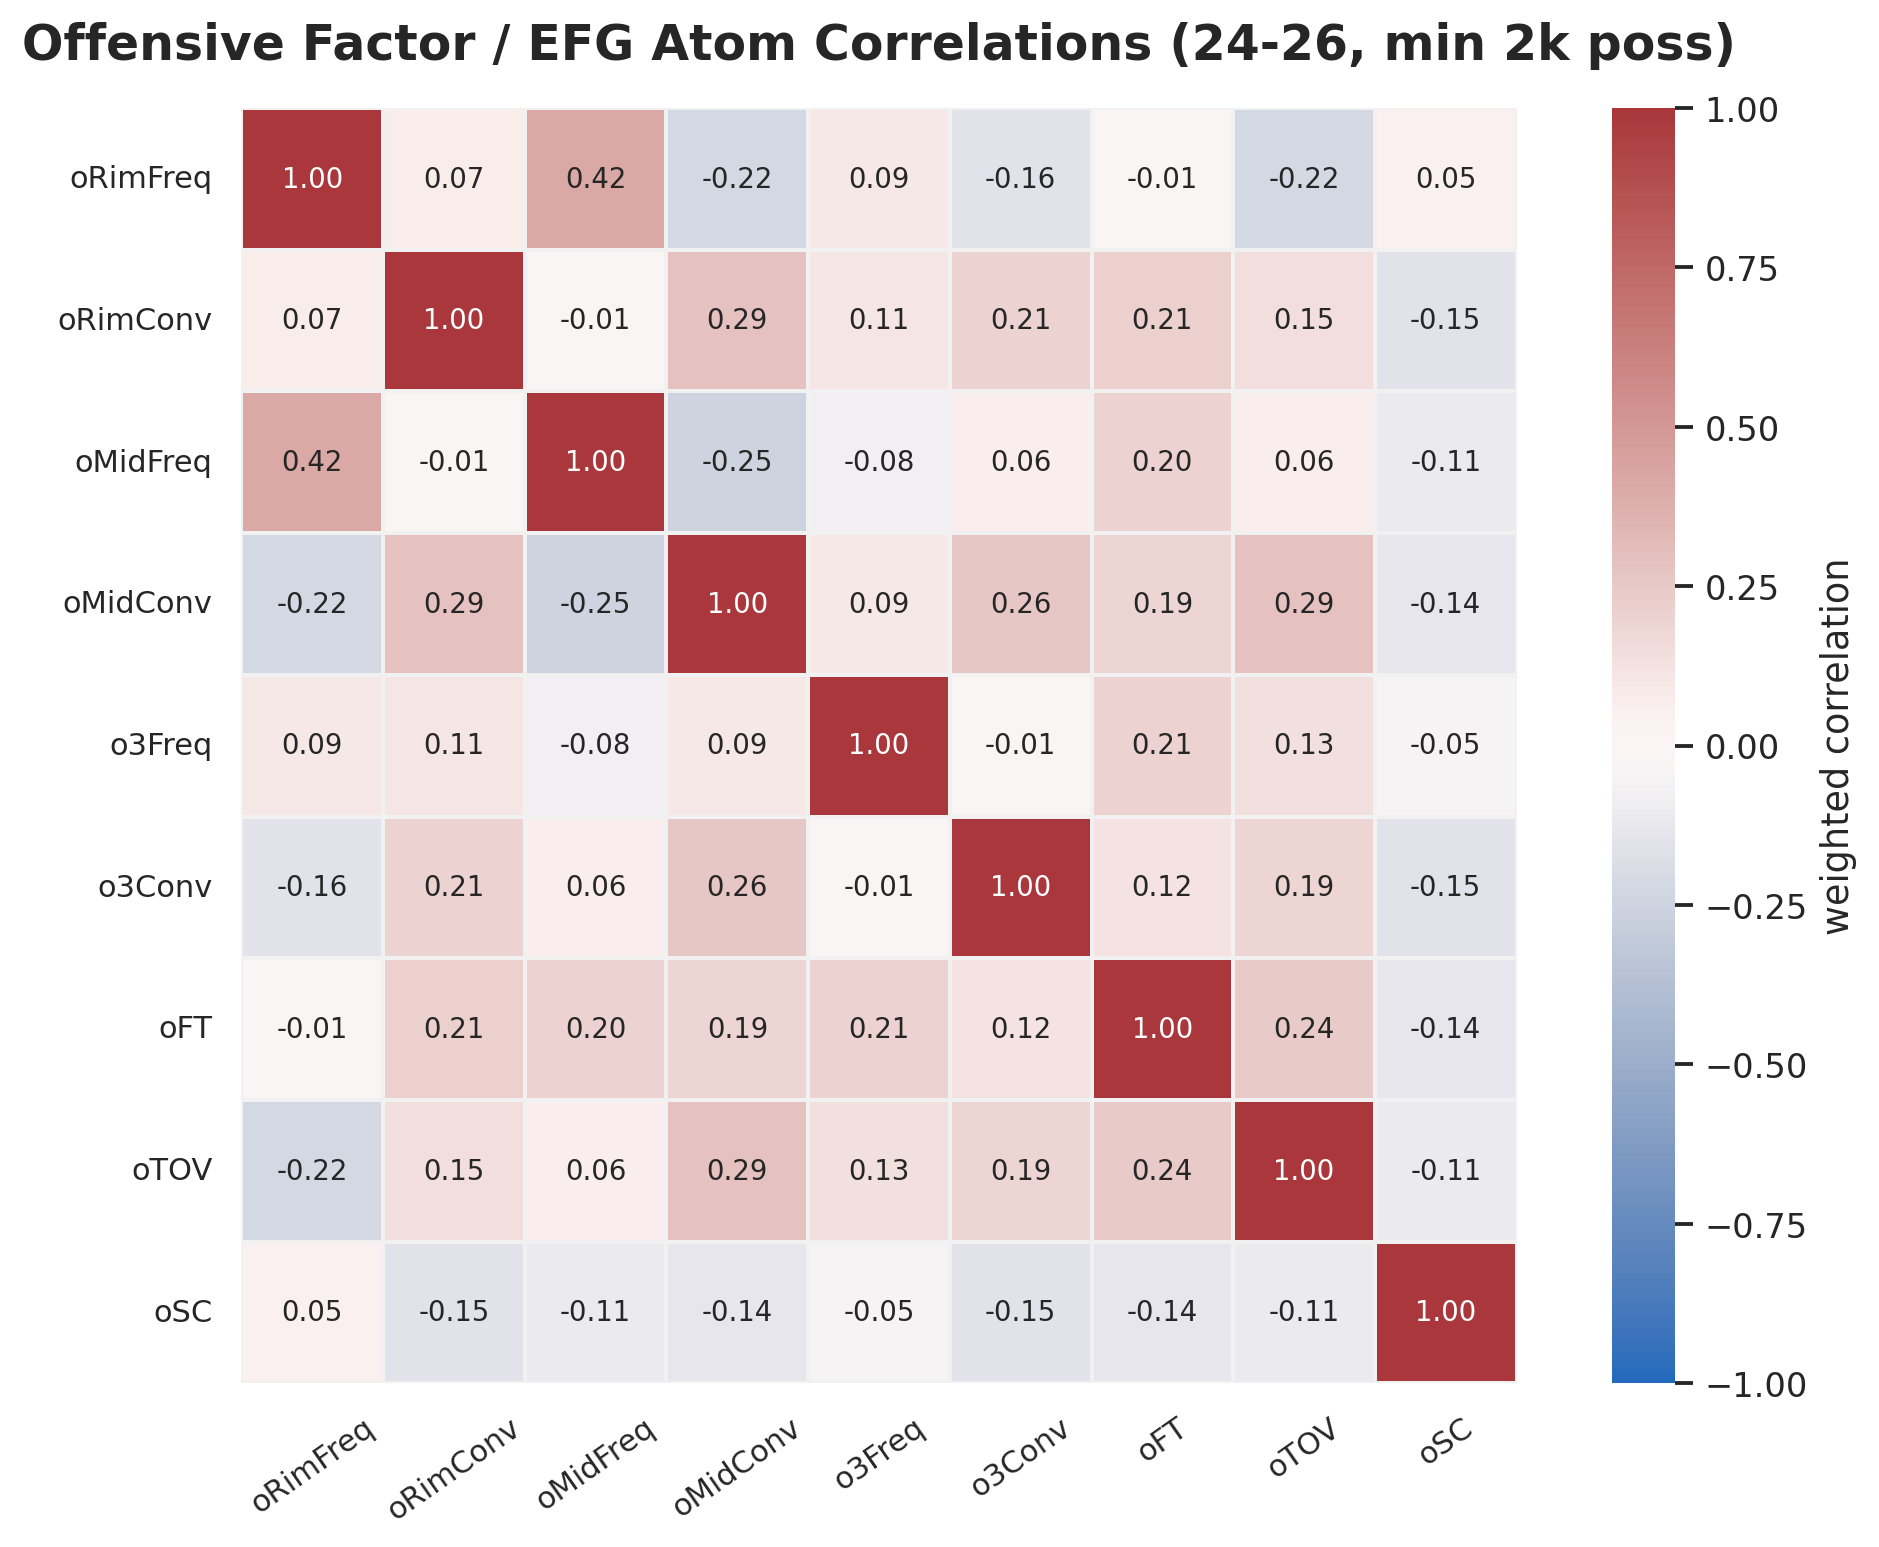
\includegraphics[width=0.88\linewidth]{figures/rapm_decomp_off_factor_corr_24_26.png}
\caption{Possession-weighted offensive factor and EFG-atom correlations,
2024--2026 players with at least 2,000 possessions.}
\label{fig:off-corr}
\end{figure}

\begin{figure}[h]
\centering
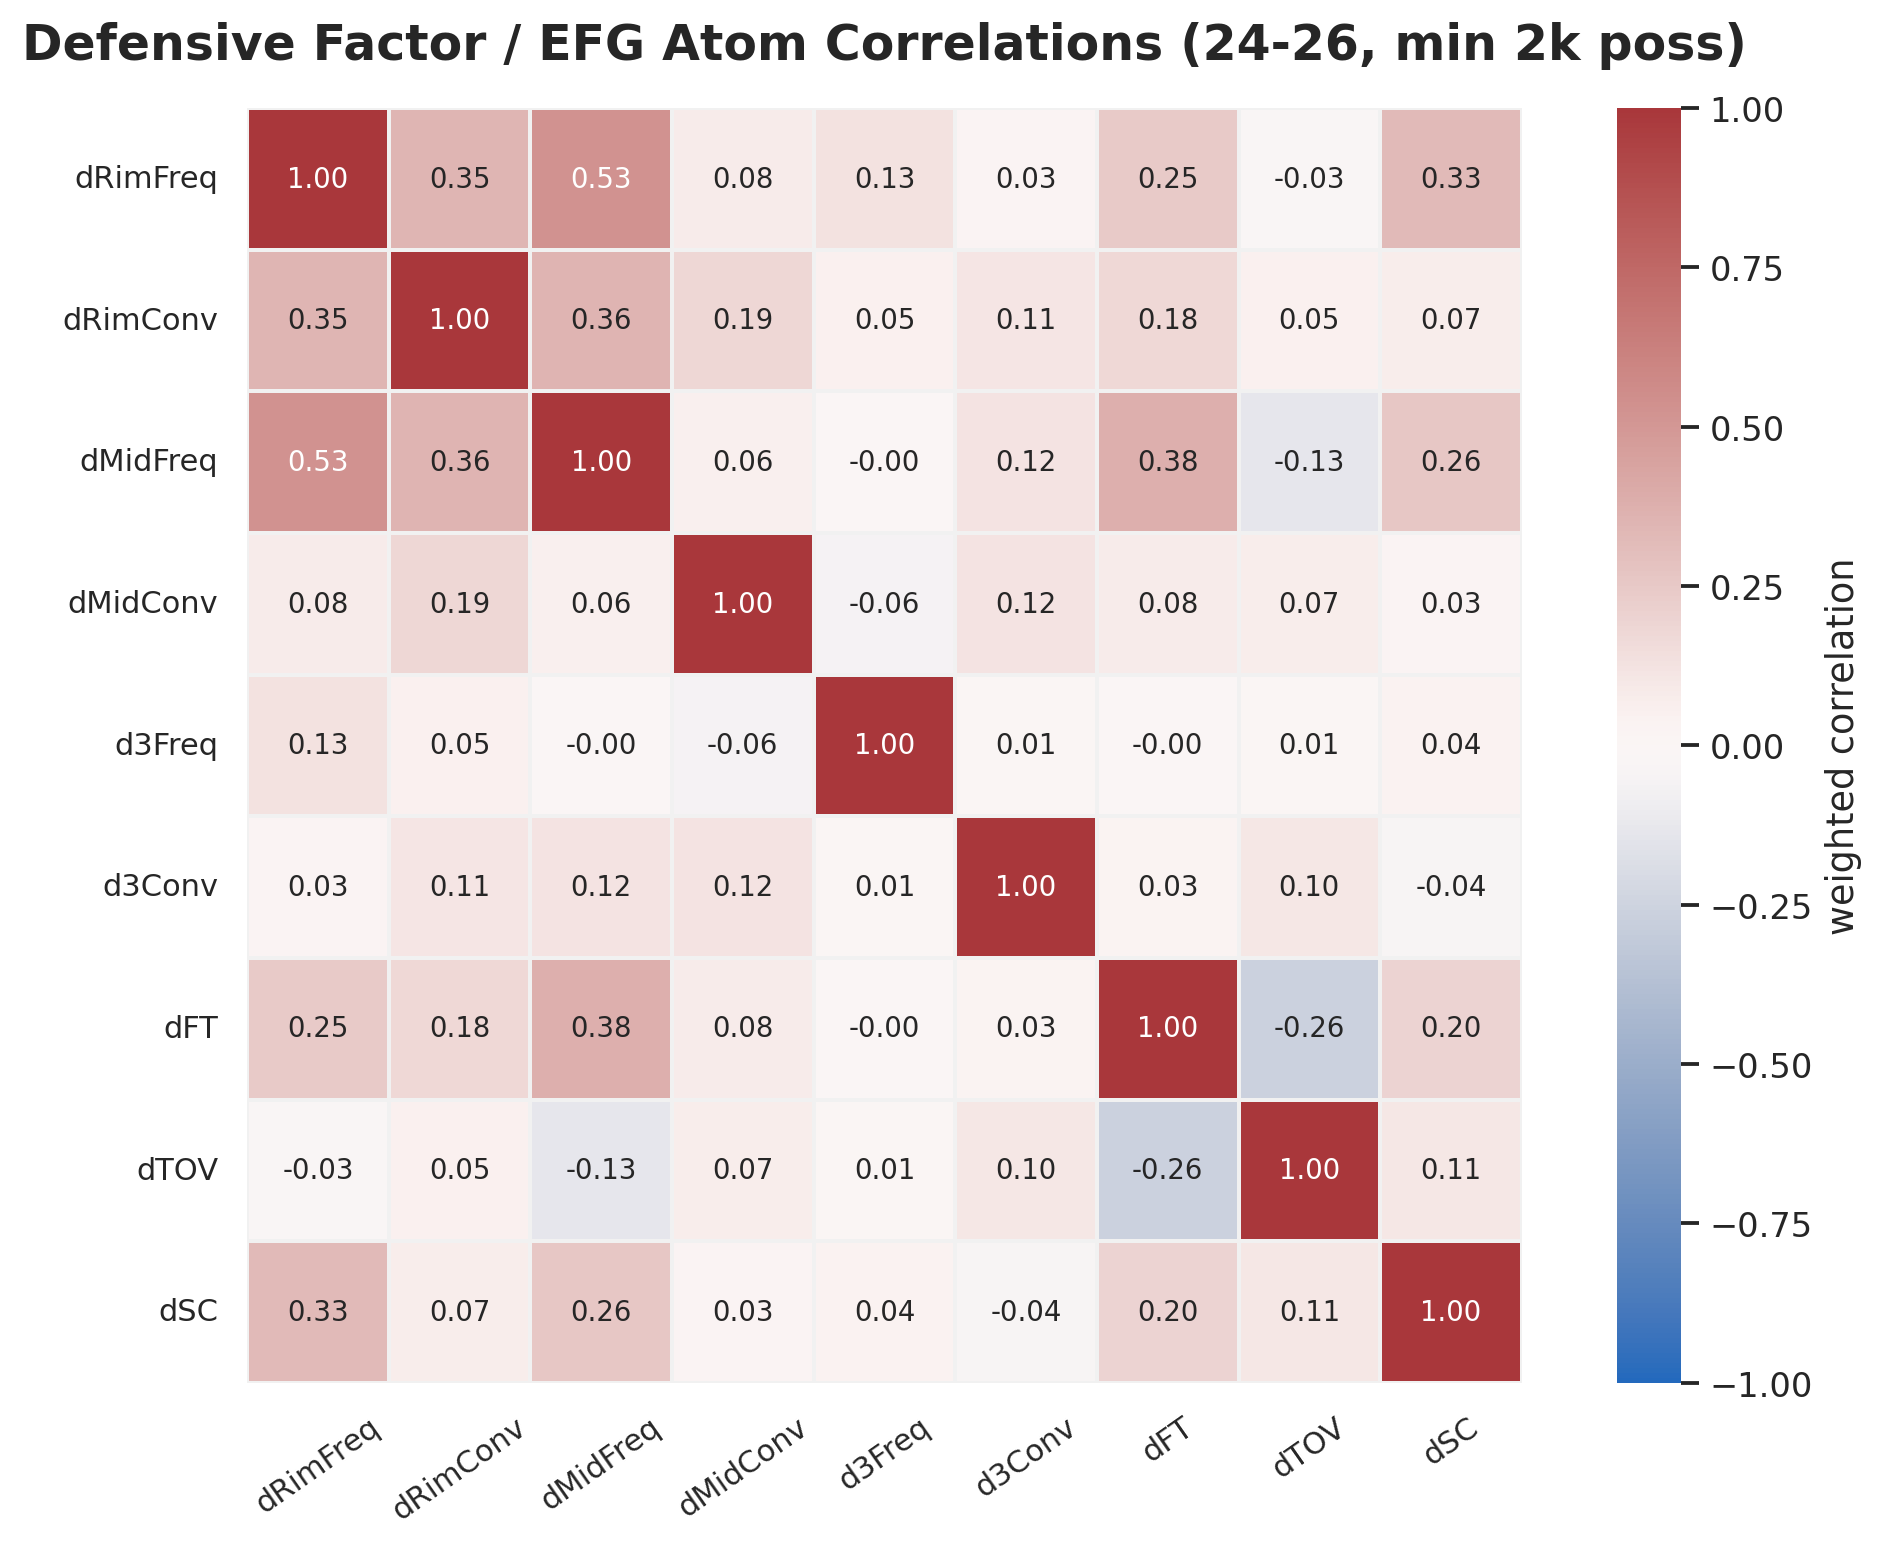
\includegraphics[width=0.88\linewidth]{figures/rapm_decomp_def_factor_corr_24_26.png}
\caption{Possession-weighted defensive factor and EFG-atom correlations,
2024--2026 players with at least 2,000 possessions.}
\label{fig:def-corr}
\end{figure}

\section{Interpretation}

RAPM DECOMP should be read as a map of where adjusted value lands, not as a
complete causal explanation of how the value was generated.  A player can
increase offensive rim value by driving, passing, screening, spacing, or simply
forcing defenses into a particular coverage.  The component says that the
adjusted lineup signal landed in rim value.  It does not say that the player
personally took every valuable rim attempt.

The same caution applies to defense.  Positive defensive shot value means the
opponent's adjusted shot value declined while the player was defending, in the
public good-positive sign convention.  It can include contests, deterrence,
scheme, opponent selection, teammate interaction, and rebounding consequences.
It is a possession-channel estimate, not a film tag.

This limitation is also the source of the metric's usefulness.  RAPM DECOMP does
not replace film or tracking analysis.  It gives them sharper targets.  Instead
of asking why a player is good in one number, an analyst can ask why the player's
lineups show high first-chance shot value, negative turnover value, or unusual
second-chance defense.

\section{Historical Coverage}

The long NBA export runs from 1997 through 2026.  That historical reach is
possible because the public shot-value decomposition uses possession, scoring,
free-throw, turnover, rebound, lineup, and shot-location information that can be
rebuilt across the long play-by-play archive.  It does not require a complete
tracking-era expected-value model for every season.

Long-window results should still be read carefully.  League shot environments
changed radically between 1997 and 2026.  A midrange frequency value in an early
2000s context and a midrange frequency value in the current NBA are measured
relative to the loaded run and nuisance-adjusted context, not relative to a
timeless league.  Season effects help, but they do not make eras identical.

The historical surface is therefore best viewed as evidence of scalability and
as a tool for audited comparison.  It is not a license to ignore era context.
The same arithmetic contract can operate across three decades; specific player
interpretations still require basketball judgment.

\section{Failure Modes}

The decomposition can fail in several ways.

First, the target identities can fail.  This is the most direct failure.  If a
child target does not add to its parent on the processed rows, then the public
story is false no matter how good the leaderboard looks.

Second, a component can be arithmetically valid but statistically unstable.
Small-sample channels, heavily collinear roles, and low-minute players can move
with ridge penalty, time decay, or window choice.  A component should not be
promoted as stable merely because it is additive.

Third, a component can be semantically too coarse.  Free-throw severity currently
combines trip type and shooter conversion.  That is a valid two-part split, but
it may not answer every foul-drawing question.  The correct response is to add a
new child identity under severity, not to overload the current term.

Fourth, users can overread the columns.  Offensive rim-frequency value is not
the player's own rim-attempt rate.  Defensive three-point conversion value is
not simply opponent luck.  The columns are adjusted possession-channel
estimates.  They are powerful only when interpreted at that level.

\section{Relation to Public Metrics}

RAPM DECOMP is not a replacement for a stable all-in-one public metric.  It is a
decomposition layer.  A product stack can have a stabilized total impact rating,
an additive RAPM DECOMP explanation underneath it, and then box-score, tracking,
and film evidence underneath each component.  The important point is that the
explanatory evidence should explain a channel whose target is already defined.

This structure is especially useful for priors.  A prior for total offense is
blunt.  A prior for rim frequency, free-throw frequency, scoring turnover value,
or second-chance defense is more precise.  The additive layer gives those priors
targets.  It also makes it harder to smuggle a box-score story into a RAPM
coefficient without stating the basketball channel being modeled.

\section{Future Work}

The first priority is stability validation.  Each component should be tested for
split-sample repeatability, predictive value, ridge sensitivity, time-decay
sensitivity, and playoff sensitivity.  Additivity is necessary for a public
decomposition, but it is not sufficient for claiming that every component is a
stable skill estimate.

The second priority is a richer shot-quality branch.  Where tracking-era
expected-value data are available, \texttt{oEFG}/\texttt{dEFG} can be split
into pre-shot expected value and making value more directly.  The current
public EFG atoms are deliberately historical and broadly available; they are not
the final form of shot-quality attribution.

The third priority is clearer public presentation.  Users should see
\texttt{oEFG}/\texttt{dEFG}, Free-Throw Value, Turnover Value, and
Second-Chance Value, with rim, midrange, and three-point atoms under the EFG
branch.  Internal solver aliases and artifact names should remain
implementation details, not the language of the public paper.

\section{Conclusion}

RAPM is valuable because it resists easy box-score stories.  But a single RAPM
coefficient can become its own mystery.  RAPM DECOMP shows that the mystery can
be reduced without abandoning adjusted plus-minus.  By defining possession-value
targets, solving them through the same lineup-adjusted ridge operator, and
publishing the actual parent coefficient alongside its factors and residual,
the method turns one impact number into a set of basketball channels that still
add back to the parent.

The claim is intentionally disciplined.  RAPM DECOMP does not solve causality,
replace film, or prove that basketball is simple.  It shows that when a public
impact metric can keep its books, it should.  In the current public exports,
actual RAPM minus the factor sum is only rounding-scale residual.  That gives
analysts a cleaner starting point: not merely who was valuable, but where the
adjusted value appeared.

\appendix

\section{Residual Definitions}

For each public player row, \texttt{off} is the actual offensive RAPM
coefficient.  The offensive decomposition residual is:
\[
\text{oRESID}
= \text{off}
- (\text{oEFG}+\text{oFT}+\text{oTOV}+\text{oSC}).
\]
The defensive side uses the public good-positive defensive sign convention:
\[
\text{dRESID}
= \text{def}
- (\text{dEFG}+\text{dFT}+\text{dTOV}+\text{dSC}).
\]
Net residual is:
\[
\text{RESID}
= \text{net\_rapm}
- (\text{off factors}+\text{def factors}).
\]

\section{Public Column Glossary}

\begin{longtable}{p{0.25\linewidth}p{0.65\linewidth}}
\toprule
Term & Meaning\\
\midrule
oEFG / dEFG & First-chance non-free-throw EFG value, after the baseline shot value is separated.\\
Rim Frequency & Value of shifting first-chance shots toward or away from rim attempts.\\
Rim Conversion & Within-rim make value after rim frequency is priced.\\
Midrange Frequency & Value of shifting first-chance shots toward or away from midrange attempts.\\
Midrange Conversion & Within-midrange make value after midrange frequency is priced.\\
Three-Point Frequency & Value of shifting first-chance shots toward or away from threes.\\
Three-Point Conversion & Within-three-point make value after three-point frequency is priced.\\
Free-Throw Value & First-chance free-throw value.\\
Trip Frequency Value & Average-value first-chance free-throw trip creation.\\
Trip Severity Value & Value above or below the average first-chance trip.\\
Turnover Value & Point-valued first-chance scoring opportunity lost on true first-chance turnovers.\\
Bad-Pass Turnover Value & Portion of turnover value assigned to bad-pass turnovers.\\
Scoring Turnover Value & Portion of turnover value assigned to other scoring or ball-handling turnovers.\\
Second-Chance Value & Post-miss scoring value in the side-level decomposition of actual RAPM.\\
\bottomrule
\end{longtable}

\section{Artifact Notes}

The empirical tables in this draft were generated from the local May 2026
pipeline outputs.  The primary public NBA surface is the 2024--2026 all-games
RAPM DECOMP weighted-factor export with score-margin adjustment, season-phase
fixed effects, and side-specific ridge penalties of 2000 and 4000.  The long
historical surface is the 1997--2026 export with the same public schema.  The
six-factor comparison uses the 2021--2026 time-decayed weighted-factor export.

\begin{thebibliography}{9}

\bibitem[Rosenbaum(2004)]{rosenbaum2004}
Dan Rosenbaum.
\newblock Measuring how NBA players help their teams win.
\newblock 82games.com, 2004.

\bibitem[Sill(2010)]{sill2010}
Joseph Sill.
\newblock Improved NBA adjusted plus-minus using regularization and
out-of-sample testing.
\newblock MIT Sloan Sports Analytics Conference, 2010.

\bibitem[Cervone et~al.(2016)]{cervone2016}
Dan Cervone, Alexander D'Amour, Luke Bornn, and Kirk Goldsberry.
\newblock A multiresolution stochastic process model for predicting basketball
possession outcomes.
\newblock \emph{Journal of the American Statistical Association}, 2016.

\end{thebibliography}

\end{document}
